% debut d'un fichier latex standard
\documentclass[a4paper,12pt,twoside]{article}
% Tout ce qui suit le symbole "%" est un commentaire
% Le symbole "\" désigne une commande LaTeX

% pour l'inclusion de figures en eps,pdf,jpg, png
\usepackage{graphicx}

% quelques symboles mathematiques en plus
\usepackage{amsmath}
\usepackage{mathenv}
%\usepackage{siunitx}

% le tout en langue francaise
\usepackage[french]{babel}

% on peut ecrire directement les caracteres avec l'accent
%    a utiliser sur Linux/Windows (! dépend de votre éditeur !)
\usepackage[utf8]{inputenc}
\usepackage[T1]{fontenc}

% pour l'inclusion de liens dans le document
\usepackage[colorlinks,bookmarks=false,linkcolor=blue,urlcolor=blue]{hyperref}

\paperheight=297mm
\paperwidth=210mm

\setlength{\textheight}{235mm}
\setlength{\topmargin}{-1.2cm} % pour centrer la page verticalement
%\setlength{\footskip}{5mm}
\setlength{\textwidth}{15.5cm}
\setlength{\oddsidemargin}{0.5cm}
\setlength{\evensidemargin}{0.5cm}

\pagestyle{plain}

% nouvelles commandes LaTeX, utilis\'ees comme abreviations utiles
\def \be {\begin{equation}}
\def \ee {\end{equation}}
\def \dd  {{\rm d}}

\newcommand{\mail}[1]{{\href{mailto:#1}{#1}}}
\newcommand{\ftplink}[1]{{\href{ftp://#1}{#1}}}
%
% latex SqueletteRapport.tex      % compile la source LaTeX
% xdvi SqueletteRapport.dvi &     % visualise le resultat
% dvips -t a4 -o SqueletteRapport.ps SqueletteRapport % produit un PostScript
% ps2pdf SqueletteRapport.ps      % convertit en pdf

% pdflatex SqueletteRapport.pdf    % compile et produit un pdf

% ======= Le document commence ici ======

\begin{document}

% Le titre, l'auteur et la date
\title{De la Terre à la Lune}
\author{Timothée Dao\\  % \\ pour fin de ligne
{\small \mail{timothee.dao@epfl.ch}}}
\date{\today}\maketitle
\baselineskip=16pt
\parindent=0pt
\parskip=12pt


\section{Introduction} %------------------------------------------

Le but de cet exercice est d'examiner la pertinence du scénario de Jules Vernes où il imagine lancer un projectile avec un canaon de la Terre à la Lune, en utilisant le schéma numérique d'Euler. On considère la gravitation de la Terre et de la Lune (en ignorant tout mouvement orbital) ainsi que la force de trainée aérodynamique du projectile. 

On a les paramètres suivants : constante gravitationnelle $G=6.674 \times 10^{-11}  \rm m^3kg^{-1}s^{-2}$, masse de la Terre $m_Z=5.972  \times 10^{24} \rm kg$, de la Lune $m_L=7.342 \times 10^{22} \rm kg$ et du projectile $m_P=1000 \rm kg$. On note la position du centre de la Terre $z_T=0$, du centre de la Lune $z_L=384'400 \times 10^{3} \rm m$, de la surface terrestre $z_0=6'378 \times 10^{3} \rm m$. \\
La force de traînée aérodynamique est $F_t=\rho SC_xv^2/2$, où $\rho_0=1.3 \rm kg/m^3$ est la densité d'air à la surface terrestre, la densité est $\rho(z)=\rho_0exp(-(z-z_0)/\lambda)$, avec $\lambda=10^4 \rm m$, $C_x=0.3$ le coefficientde traînée aérodynamique et $S=\pi R^2$ la surface de la section du projectile, approximée par un disque de rayon $R=0.5 \rm m$.

Les expressions des trois forces à prendre en compte sont les suivantes :
\be \label{ForceTerre} 
F_{g_T}=-G \frac{m_P m_T}{z^2} e_z
\ee
\be \label{ForceLune} 
F_{g_L}=-G \frac{m_P       m_L}{(z-z_L)^2} e_{z-z_L}
\ee
\be \label{ForceTrainee}
F_t=-\frac{1}{2} \rho_0 exp{(-\frac{z-z_0}{\lambda})} \pi R^2 C_x v^2  e_v
\ee
où $e_x=\frac{x}{\lvert x \rvert}$ donne à chaque fois le sens de la force.

\section{Calculs analytiques}

\subsection{Équations différentielles}
En utilisant la 2ème loi de Newton, $\vec{F}=m \vec{a}$, et en projetant sur l'axe $z$ on obtient 
\be
\frac{\dd }{\dd t} 
\left( \begin{array}{c} v \\ z \end{array} \right)
=
\left( \begin{array}{c}
    -G(\frac{m_T}{z^2}e_z+\frac{m_L}{(z-z_L)^2}e_{z-z_L}) - \frac{1}{2} \rho_0 exp{(-\frac{z-z_0}{\lambda})} \pi R^2 C_x v^2  e_v\\
     v
\end{array} \right)
\ee
avec les conditions initiales 
\be 
\left( \begin{array}{c} v(0) \\ z(0) \end{array} \right) 
=
\left( \begin{array}{c} v_0 \\ z_0 \end{array} \right)
\ee


\subsection{Position d'équilibre $z_E$}
On cherche à trouver la position d'équilibre $z=z_E$ où la résultante des forces gravitationnelles s'annulle.
Cela se résume à résoudre l'équation 
\[ F_{g_T}(z_E)+F_{g_L}(z_E)=0 \]
\[ \Leftrightarrow G\frac{m_Pm_T}{{z_E}^2}=G\frac{m_Pm_L}{(z_E-z_L)^2}  \Leftrightarrow (\frac{z_L-z_E}{z_E})^2=\frac{m_L}{m_T} \]
\be \Leftrightarrow z_E=\frac{z_L}{1+\sqrt{\frac{m_L}{m_T}}} \ee
En utilisant les données numériques, on obtient $z_E=346'037 \times 10^3  \rm m$.
\footnote{\textit{Remarque : on a exclu l'autre solution $z_E=\frac{z_L}{1-\sqrt{\frac{m_L}{m_T}}}$ car les deux forces sont de même intensité mais aussi dans le même sens à cette position, elles ne s'annulent donc pas.}}



\subsection{Vitesse initiale $v_0$ pour atteindre $z_E$}
En ignorant l'atmosphère ($\rho_0=0$), on cherche à trouver la vitesse $v_0$ que doit avoir le projectile en $z=z_0$ pour qu'il puisse juste atteindre le point d'équilibre $z=z_E$ (i.e. avec une vitesse nulle à cet endroit).

En absence de la force de traineée, il ne reste que des forces conservatives ($\vec{F}_{g_{T,L}}$) et donc l'énergie mécanique du projectile est conservée : $E_{mec} = E_{pot} + E_{cin} = const$. On en tire 
\[ E_{pot,i} + E_{cin,i} = E_{pot,f} + E_{cin,f} \]
\[ \Leftrightarrow Gm(\frac{m_T}{z_0}+\frac{m_L}{z_L-z_0})+\frac{1}{2}m{v_0}^2 = Gm(\frac{m_T}{z_E}+\frac{m_L}{z_L-z_E})\]
\be \Leftrightarrow v_0= \sqrt{2G}(\frac{m_T}{z_0}+\frac{m_L}{z_L-z_0}-\frac{m_T}{z_E}-\frac{m_L}{z_L-z_E}) \ee

En utilisant les données numériques, on obtient $v_0=11065.71228 \rm m/s$.

\section{Simulations numériques}
\subsection{Cas sans atmosphère $(\rho_0=0)$}
On simule ici un voyage de 24 heures, $t_{fin}=86'400\rm s$. On effectue un série de simulations à partir de la condition initiale $z(0)=z_0$, $v(0)=v_0$ et pour $n_{steps}=$ 1000, 2000, 4000, 8000, 16000, 32000. On obtient ainsi les résultats montrer sur la FIG.\ref{convSans}. Nous avons utilisé le schéma d'Euler qui est d'ordre 1 et nous obtenons comme attendu une droite lorsqu'on plot la position (ou la vitesse) finale en fonction de $\Delta t = \frac{t_{fin}}{n_{steps}}$
\begin{figure} %------------------------------------------------
\begin{center}
\includegraphics[width=0.49 \textwidth]{../q1_3_a/convPsans}
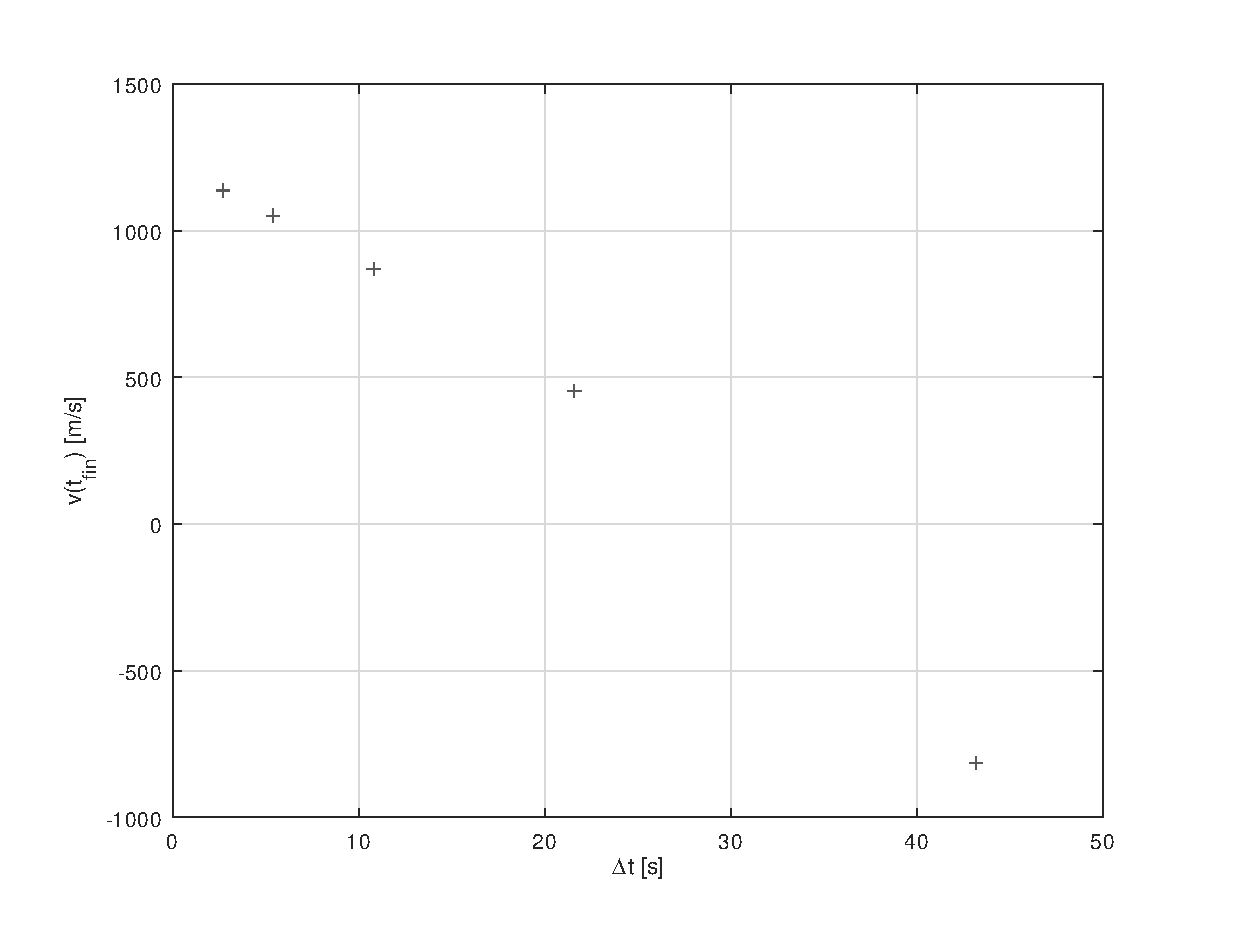
\includegraphics[width=0.49 \textwidth]{../q1_3_a/convVsans}
\end{center}
\caption{\em \label{convSans} Position et vitesse finales en fonction de $\Delta t$, il est clair que les deux suivent une loi linéaire.}
\end{figure} %---------------------------------------------------


\subsection{Cas avec atmosphère $(\rho_0=1.3 \rm kg/m^3)$}
On veut maintenant simuler la traversée de l'atmosphère, on doit donc prendre en compte la force de traînée aérodynamique  (avec $\rho_0 =1.3 \rm kg/m^3$). Nous prenons pour temps final $t_{fin}=10 \rm s$ et les mêmes conditions initiales que précédemment ($z_0$, $v_0$). On effectue les simulations avec $n_{steps}=$ 200, 400, 800, 1600, 3200, 6400. Comme précédemment, on s'attend à ce que la position finale et la vitesse finale soient linéairement dépendants de $\Delta t$, et c'est effectivement ce qu'on observe sur la FIG.\ref{convAvec}.
\begin{figure} %------------------------------------------------
\begin{center}
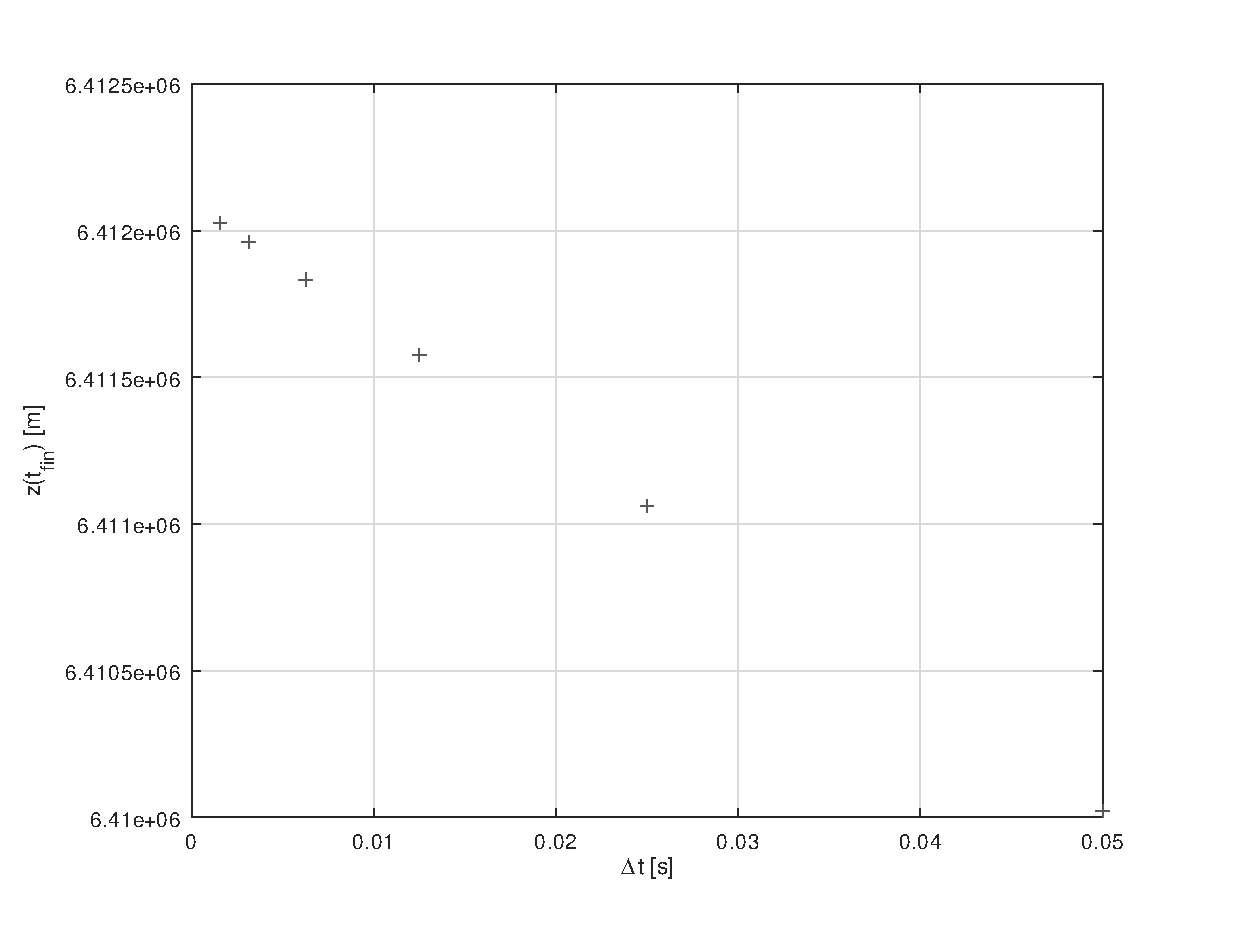
\includegraphics[width=0.49 \textwidth]{../q1_3_b/convPavec}
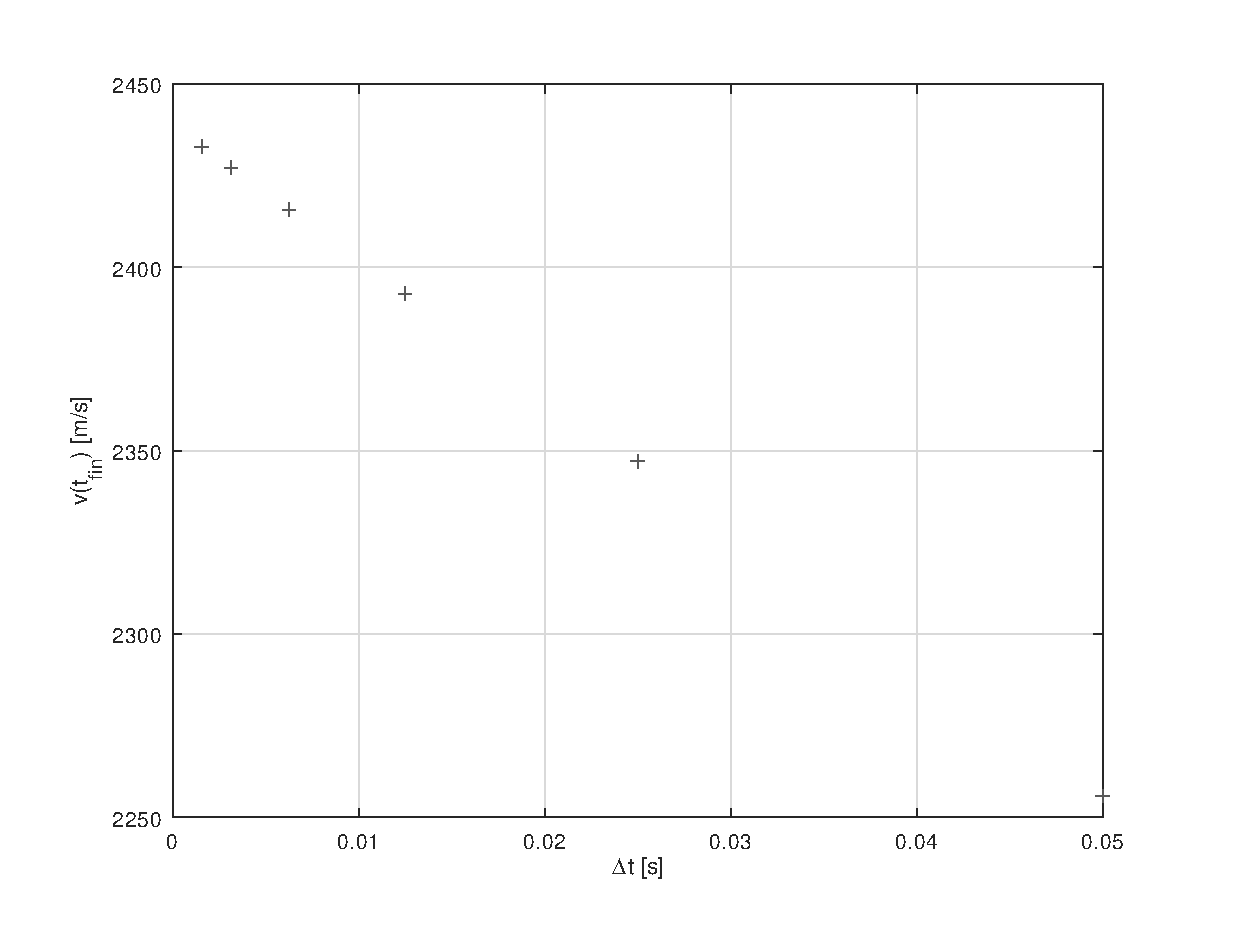
\includegraphics[width=0.49 \textwidth]{../q1_3_b/convVavec}
\end{center}
\caption{\em \label{convAvec} Position et vitesse finales en fonction de $\Delta t$, il est clair que les deux suivent une loi linéaire.}
\end{figure} %---------------------------------------------------


\subsection{Recherche de vitesses initiales $v_0$}
Dans le cas sans atmosphère, on cherche la vitesse initiale pour atteindre le centre de la Lune en 97h20min. On utilise la méthode de la dichotomie avec $n_{steps}=$ 32000, 64000, 128000, 256000, 512000, 1024000. De plus, dans le cas avec atmosphère, on cherche également la vitesse initiale que doit avoir le projectile pour qu'il ait une vitesse de 11km/s après la traversée de l'atmosphère (après 10s). On utilise également la méthode de la dichotomie avec $n_{steps}=$ 3200, 6400, 12800, 25600, 51200, 102400. Les résultats sont montrés sur la FIG.\ref{convV0} et nous pouvons extrapoler ces résultats dans la limite $\Delta t \rightarrow 0$ (dans la mesure où les résultats suivent une loi linéaire) et nous trouvons $v_{0_{Lune}}=11074 \rm m/s$ et $v_{0_{atmo}}=51300 \rm m/s$.
\begin{figure} %------------------------------------------------
\begin{center}
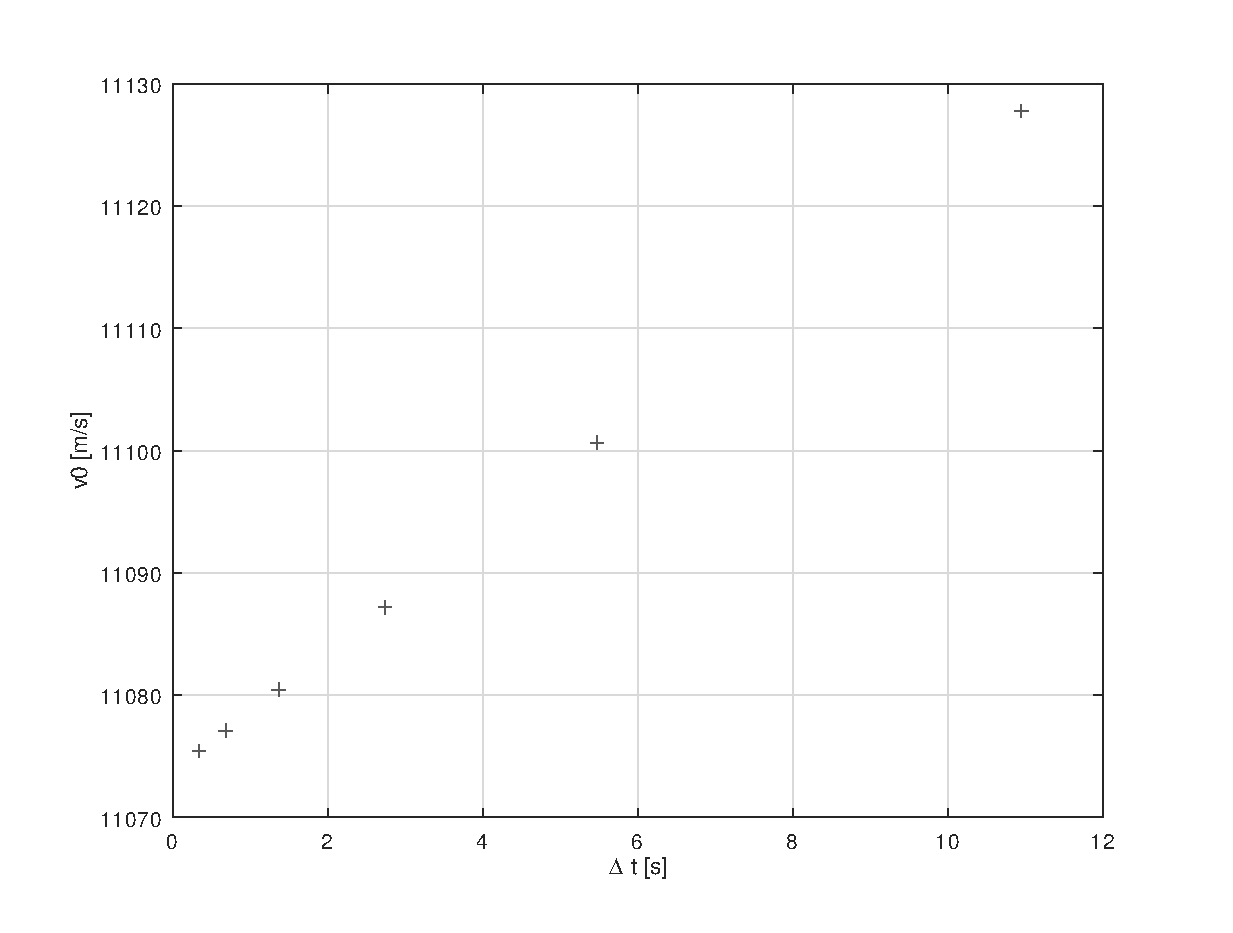
\includegraphics[width=0.49 \textwidth]{../q1_3_c/convV0sans}
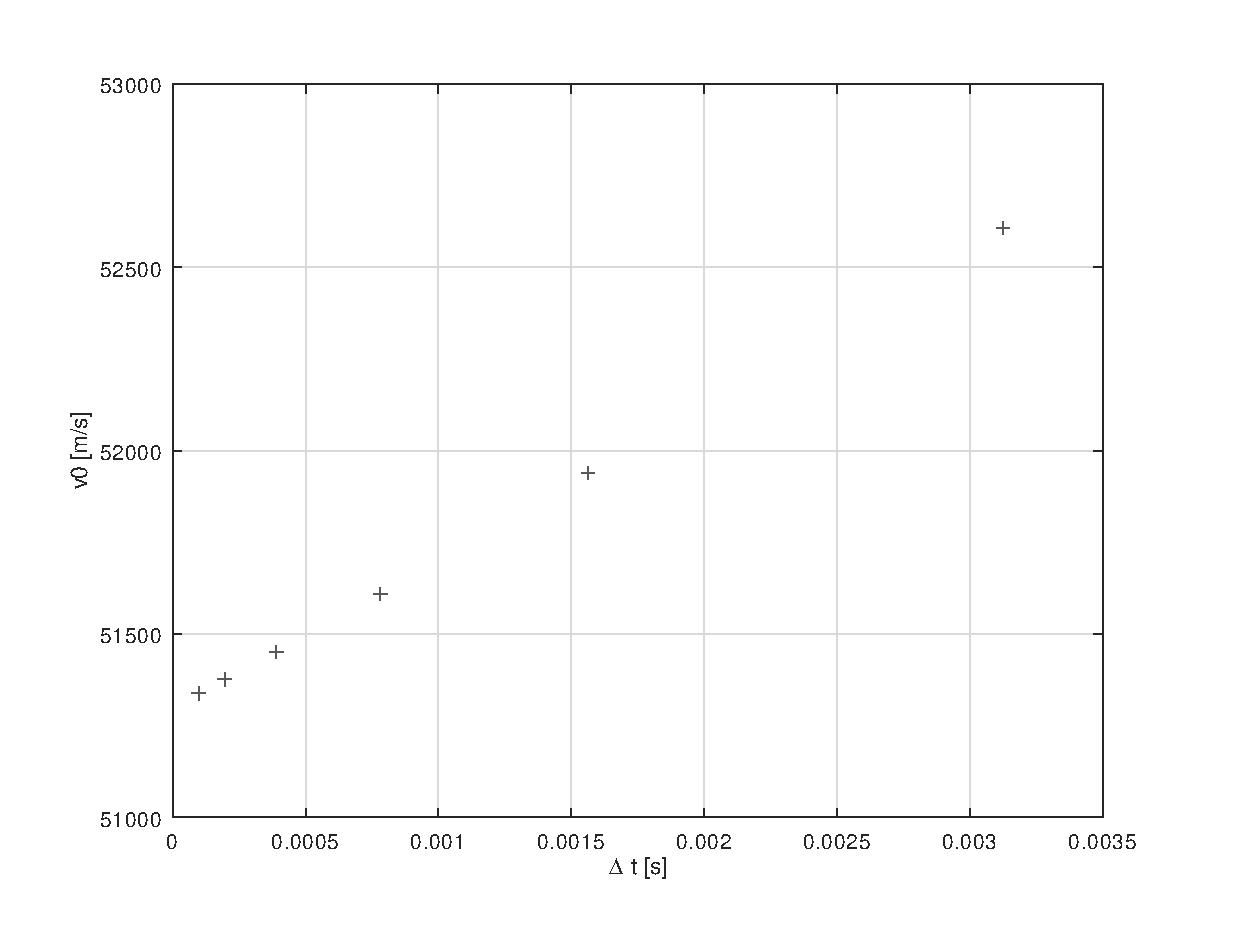
\includegraphics[width=0.49 \textwidth]{../q1_3_c/convV0avec}
\end{center}
\caption{\em \label{convV0} Position et vitesse finales en fonction de $\Delta t$, il est clair que les deux suivent une loi linéaire.}
\end{figure} %---------------------------------------------------


%On fait r\'ef\'erence \`a la FIG.\ref{figPlot} avec la commande
%\verb|\ref{fig:Plot}|.

\end{document} %%%% THE END %%%%
